\documentclass[border=10pt]{standalone}
\usepackage[svgnames]{xcolor}
\usepackage{amsmath}
\usepackage{pgfplots}
\pgfplotsset{compat=newest}
\usepackage[sfdefault]{FiraSans}
\usepackage{FiraMono}
\renewcommand*\familydefault{\sfdefault}
\begin{document}
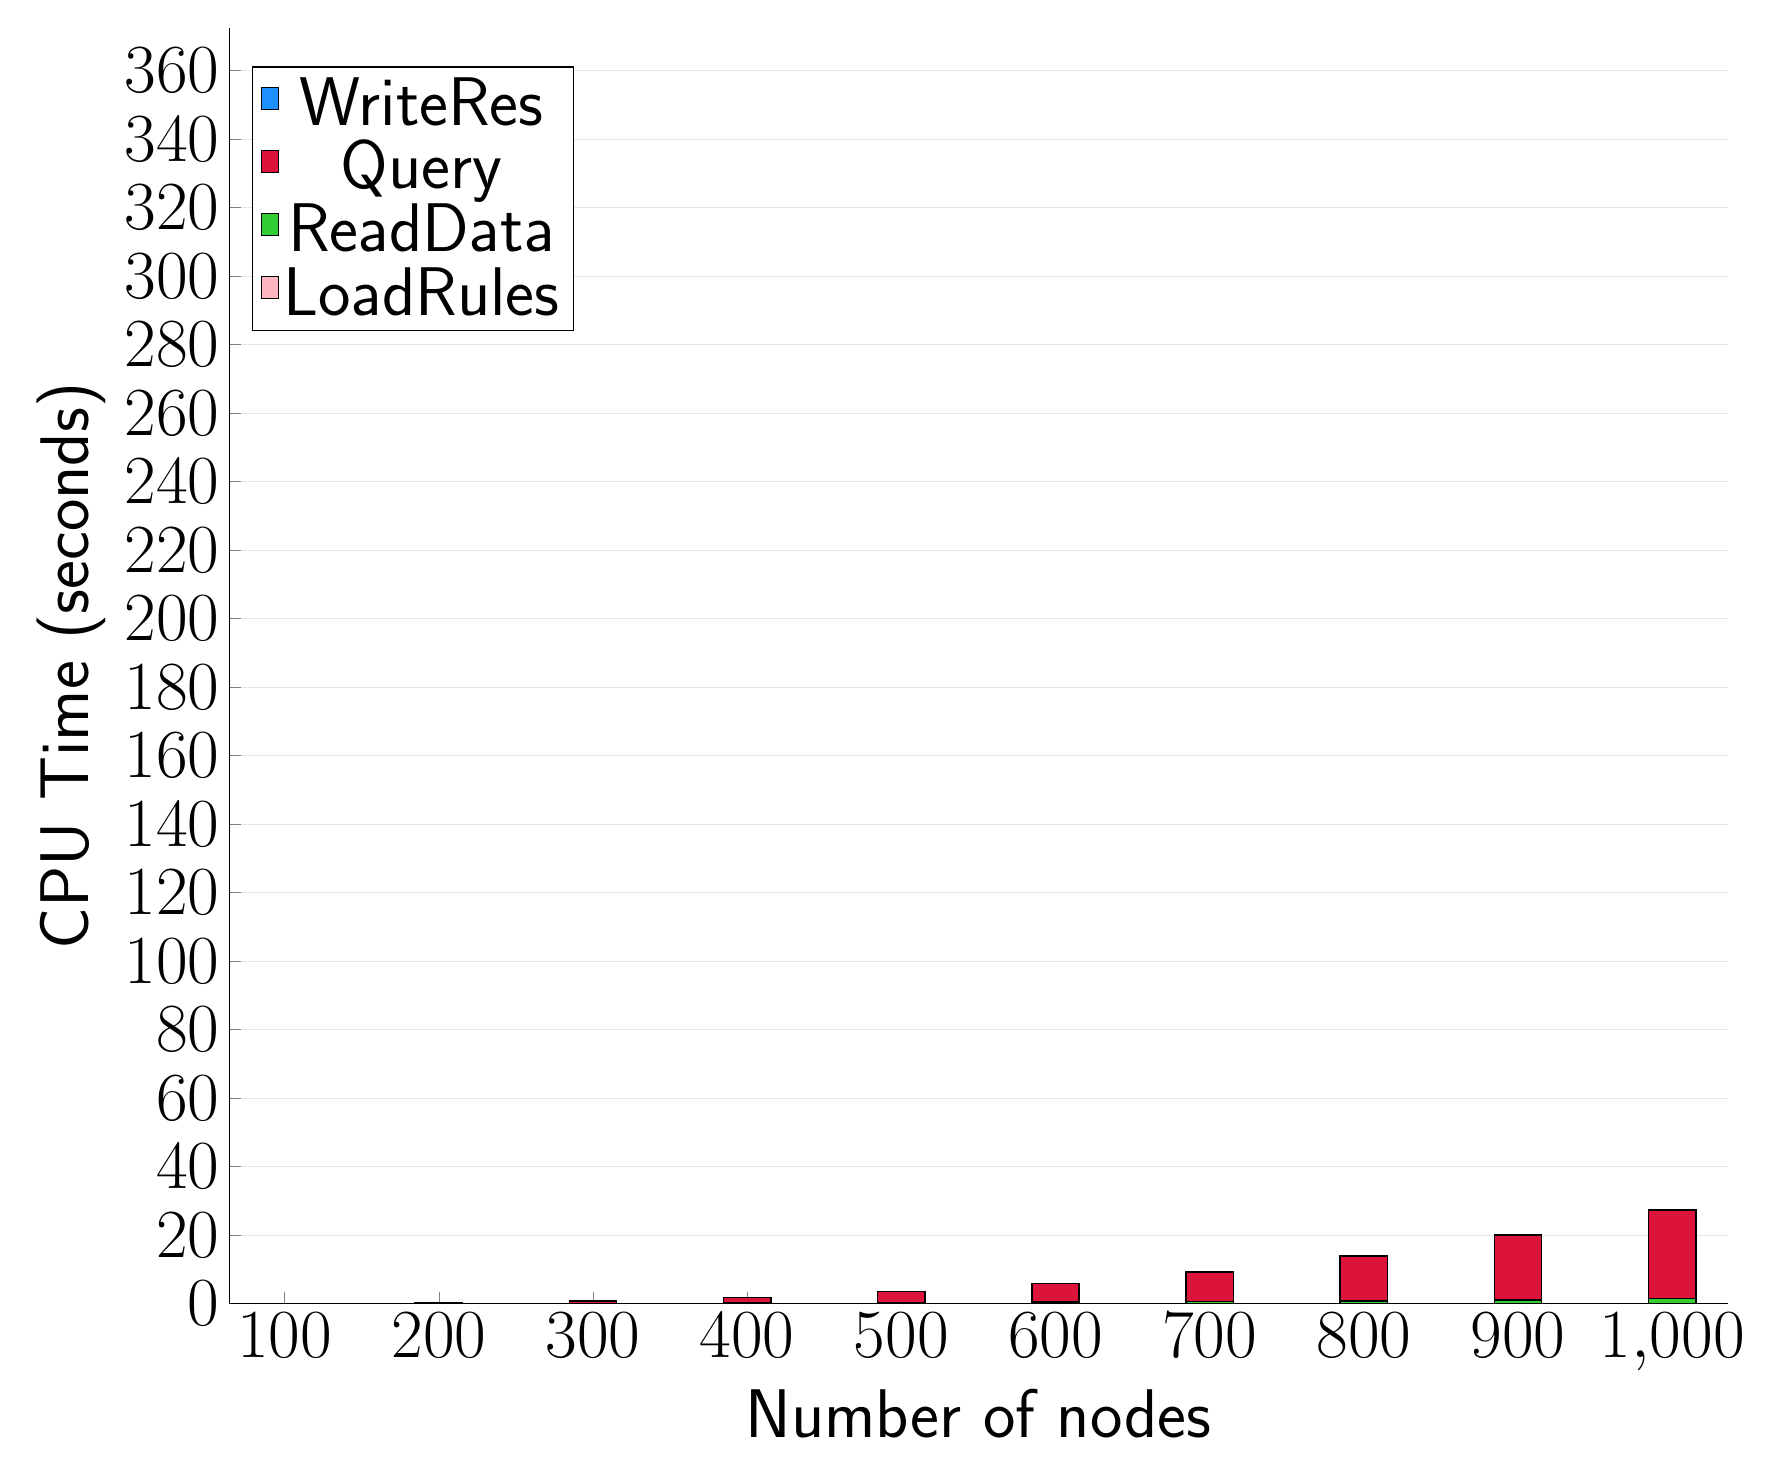
\begin{tikzpicture}
\begin{axis}[
   ybar stacked,
   width=1.7\textwidth,
   bar width=0.6cm,
   ymajorgrids, tick align=inside,
   major grid style={draw=gray!20},
   xtick=data,
   ymin=0, ymax=372.4108,
   axis x line*=bottom,
   axis y line*=left,
   enlarge x limits=0.04,
   legend style={
       at={(0.23, 0.97)},
       anchor=north east,
       legend columns=1,
       font=\Huge,
   },
   ylabel={CPU Time (seconds)},
   xlabel={Number of nodes},
   label style={font=\Huge},
   tick label style={font=\Huge},
]
\addlegendimage{fill=DodgerBlue, draw=black, line width=0.2pt}
\addlegendentry{WriteRes}
\addlegendimage{fill=Crimson, draw=black, line width=0.2pt}
\addlegendentry{Query}
\addlegendimage{fill=LimeGreen, draw=black, line width=0.2pt}
\addlegendentry{ReadData}
\addlegendimage{fill=LightPink, draw=black, line width=0.2pt}
\addlegendentry{LoadRules}
\addplot +[fill=LightPink, draw=black, line width=0.55pt] coordinates {
(100, 0.0006207999999999996)
(200, 0.0005174000000000001)
(300, 0.0005399999999999999)
(400, 0.0005340000000000006)
(500, 0.0005485999999999996)
(600, 0.0005659999999999993)
(700, 0.0005516)
(800, 0.0005531999999999998)
(900, 0.0005592000000000001)
(1000, 0.0005686000000000004)
};
\addplot +[fill=LimeGreen, draw=black, line width=0.55pt] coordinates {
(100, 0.008504600000000001)
(200, 0.034625)
(300, 0.0838918)
(400, 0.1596292)
(500, 0.2690478)
(600, 0.4140522000000001)
(700, 0.5932308)
(800, 0.8259252)
(900, 1.1294066)
(1000, 1.5037904000000002)
};
\addplot +[fill=Crimson, draw=black, line width=0.55pt] coordinates {
(100, 0.027246)
(200, 0.2112002)
(300, 0.6991479999999999)
(400, 1.6636803999999998)
(500, 3.2458600000000004)
(600, 5.484289)
(700, 8.7106784)
(800, 13.0839268)
(900, 18.8932268)
(1000, 25.756134000000003)
};
\addplot +[fill=DodgerBlue, draw=black, line width=0.55pt] coordinates {
(100, 0.0005281999999999995)
(200, -0.0009503999999999957)
(300, -0.007310600000000012)
(400, -0.001468199999999964)
(500, 0.016644799999999994)
(600, -0.011876999999999782)
(700, -0.01639760000000017)
(800, 0.0019817999999997226)
(900, -0.2094853999999998)
(1000, -0.04742680000000092)
};
\end{axis}
\end{tikzpicture}

\end{document}
